\subsubsection{Adapt PLM} %Pre-trained Language Models
\label{sec:adaptplm}

\begin{figure}[H]
    \centering
    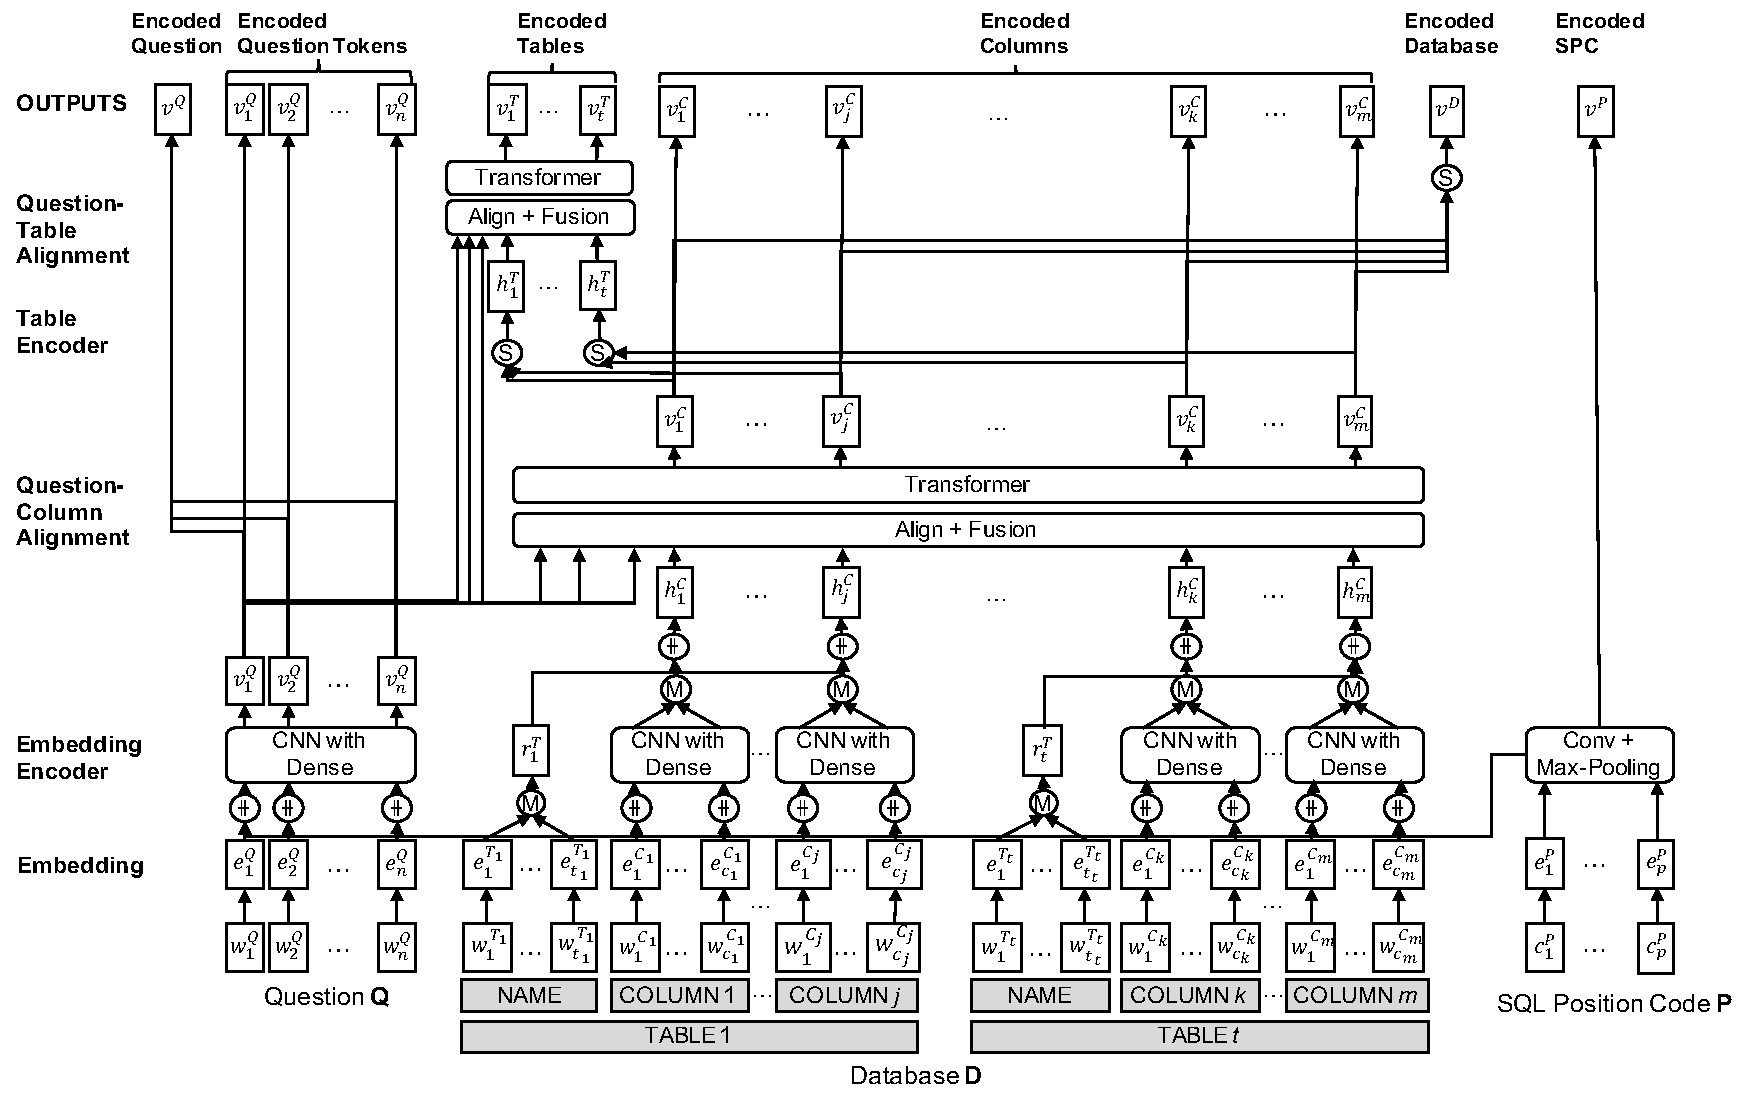
\includegraphics[width=\textwidth]{pics/enc/fig_encode}
    \caption{Network architecture of the proposed input encoder. \raisebox{-0.5ex}{
\includegraphics[height=3.3mm]{pics/enc/mark_1}} represents vector concatenation, \raisebox{-0.5ex}{
\includegraphics[height=3.3mm]{pics/enc/mark_2}} represents max-pooling and \raisebox{-0.5ex}{
\includegraphics[height=3.3mm]{pics/enc/mark_3}} represents self-attention.\cite{choi_ryansql_2020}}
    \label{fig:ryan}
\end{figure}

Adapt \ac{PLM} methods aim to utilize the knowledge encapsulated in pre-trained language models, such as BERT\cite{DBLP:journals/corr/abs-1810-04805}, to improve their performance on text-to-SQL tasks. These methods modify or extend the original PLMs to better align with the specific requirements of the task.

One common approach is to encode both the natural language questions and the database schemas using PLMs. For instance, SQLova\cite{DBLP:journals/corr/abs-1902-01069} and RYANSQL\cite{10.1162/coli_a_00403} concatenate the question words and schema words as input to the BERT encoder. This approach allows the model to learn representations that capture the relationships between questions and the underlying schema. In figure \ref{fig:ryan}, the authors of RYANSQL\cite{10.1162/coli_a_00403} propose a novel encoder that combines the BERT encoder with a self-attention mechanism to capture the interactions between the question and schema words. As you can see it passes the question words and database tables schemas through embedding layers, then concatenates them and passes them through the BERT encoder. The output of the BERT encoder is then passed through a self-attention layer to capture the interactions between the question and schema words. The self-attention layer is then concatenated with the BERT encoder output and passed through a feed-forward network to produce the final representation of the question and schema.

Some methods go a step further by adjusting the embeddings produced by the PLMs. X-SQL\cite{he2019xsql} proposes the replacement of the segment embeddings from the pre-trained encoder with column-type embeddings for the WikiSQL dataset. Guo and Gao \cite{guo2020content} introduce an approach that encodes additional feature vectors for matching between question tokens and table cells, as well as column names. These feature vectors are then concatenated with the BERT embeddings of questions and DB schemas.

HydraNet\cite{lyu_hybrid_2020} uses BERT to encode the question and individual columns, an approach that is more aligned with the tasks BERT is pre-trained on. After obtaining BERT representations for all columns, the model selects the top-ranked columns for SQL prediction


\begin{table}[t]
    \centering
    \scalebox{0.8}{
        \begin{tabular}{lcc}
            \toprule
            \textbf{Model}                                  & \textbf{Execution Accuracy} \\
            Seq2SQL\cite{zhong_seq2sql_2017}                & 60.8                        \\
            TypeSQL\cite{DBLP:journals/corr/abs-1804-09769} & 74.5                        \\
            \midrule
            SQLova\cite{DBLP:journals/corr/abs-1902-01069}  & 90.2                        \\
            Guo\cite{guo2020content}                        & 91.1                        \\
            HydraNet\cite{lyu_hybrid_2020}                  & 92.4                        \\
            \bottomrule
        \end{tabular}
    }
    \caption{The execution accuracy on the WikiSQL dev set.}
    \label{table:methods:encoders:adaptplm}
\end{table}

Examining the WikiSQL benchmark results in Table \ref{table:methods:encoders:adaptplm}, we can observe a significant overall performance improvement when employing pre-trained language models (PLMs) compared to previous methods. This enhancement can be attributed to the ability of PLMs, such as BERT, to capture complex linguistic patterns and relationships within the input data. By leveraging the knowledge encapsulated in these models and adapting them to the text-to-SQL task, researchers have been able to achieve better alignment with the specific requirements of the problem domain. As a result, PLM-based approaches have demonstrated superior performance in generating accurate SQL queries from natural language questions, surpassing traditional methods and showcasing the potential of PLMs in addressing complex language understanding tasks.
